\section{Versuchsaufbau/-durchführung}
Die Brennweite einer Linse wird im Versuch $V408$ auf drei
verschiedene Weisen bestimmt.
Die Verfahren werden im Folgenden kurz erklärt.

Als Lichtquelle wird eine Halogenlampe verwendet und als
Gegenstand ein \emph{Perl L}. Mit Hilfe eines Schrimes wird
das gebrochene Licht sichtbar gemacht werden.

\subsection{Bestimmung der Brennweite mit der Linsengleichung}

Der Schirm, die Linse, das Perl L und die Lampe werden auf einer
Geraden plaziert.
Man verändert die Bildweite $b$ solang, bis ein schrafes Bild auf dem
Schirm zu erkennen ist. Das Wertepaar ($b$,$g$) werden notiert.
Danach verändert man die Position der Linse und stellt den Schirm neu ein.
Das Wertepaar wird wieder vermerkt. Dieser Vorgang wird solang wiederholt, bis
zehn Wertepaare erfasst worden sind.
Mit Hilfe der Linsengleichung \eqref{eq: linsengleichung} und den Wertepaaren kann, dann die
Brennweite $f$ bestimmt werden.

\subsection{Bestimmung der Brennweite mit der Methode von Bessel}
Um die Methode von Bessel zu verwenden, lässt man die Entfernung zwischen
Gegenstand und Bild fest. Man verschiebt die Linse nun solang, bis zwei
Positionen gefunden worden sind, bei den ein scharfes Bild auf dem Schirm erkennbar ist.
Man erhält zwei Wertepaare ($b_1$,$g_1$) und ($b_2$,$g_2$).
Mit Hilfe der Hilfsgrößen $e=g_1+b_1=g_2=b_2$ und $d=g_1-b_1=g_2-b_2$ und der Formel
\begin{equation}
  \label{eq: bessel_methode}
  f=\frac{e^2-d^2}{4e}
\end{equation}
ist eine Berechung der Brennweite möglich.
Nach dem Aufnahme der Wertepaare, wird die Linse neu positioniert.
Der Vorgang wird zehn Mal wiederholt.

Zusätzlich soll die chromatische Abberation der Linse untersucht werden,
dazu werden je fünf Wertepaare für rot und blau gefiltertes Filter
aufgenommen.
\subsection{Bestimmung der Brennweite mit der Methode von Abbe}
Die Methode von Abbe wird verwendet, um die Brennweite und die Lage der Hauptebenen
eines Linsensystems zu bestimmen. Hierzu wird der Abbildungsmaßstab $V$,
die Gegenstands- und Bildweite verwendet. Da die Hauptebenen nicht bekannt sind,
werden die Weiten $g'$ und $b'$ zu einem gewählten Punkt $A$ gemessen. Es gilt der Zusammenhang
\begin{align}
    g'=g+h=f\left(1+\frac{1}{V}\right)+h \label{eq: abstaende_abbe_g} \\
    b'=b+h'=f\left(1+V\right)+h' \label{eq: abstaende_abbe_b}
\end{align}
Als Linsensystem wird eine Zerstreungs- und Sammellinse verwendet (vgl. Abbildung \ref{fig: linsensystem}).
\begin{figure}
    \centering
    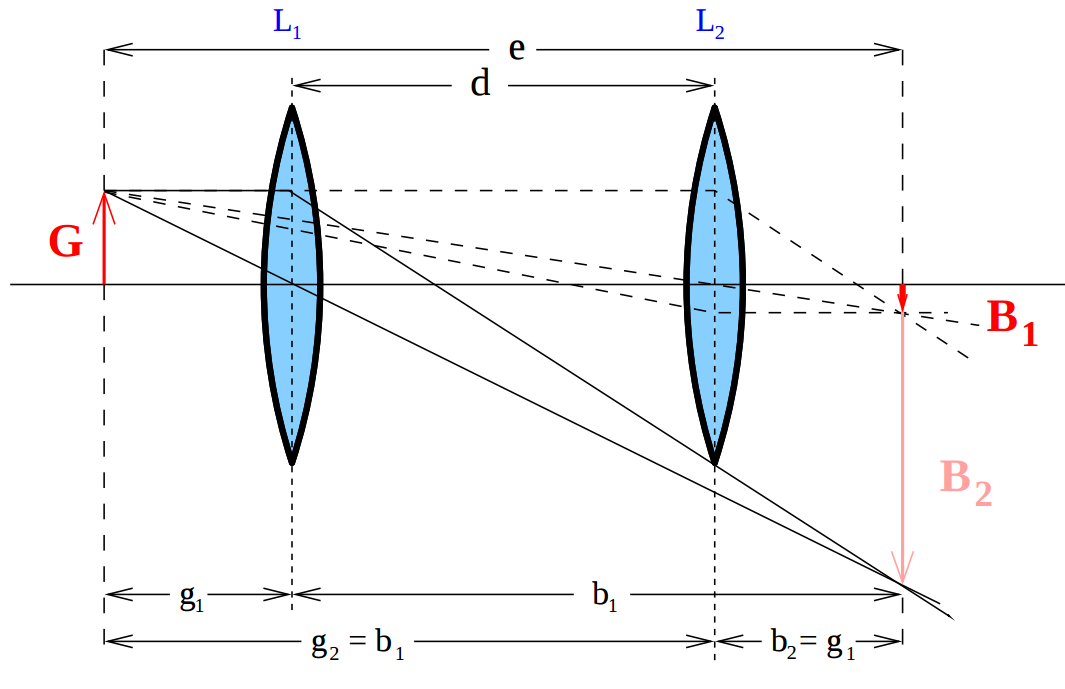
\includegraphics[width=0.6\textwidth]{./pics/linsensystem.png}
    \caption{Linsensystem \cite{anleitung408}.}
    \label{fig: linsensystem}
\end{figure}
Die relativen Bild- und Gegenstandsweiten werden von der Mittelebene
der Sammellinse gemessen.
Es wird der Schrim, bei fester Linsenposition, solang verschoben bis ein schrafes
Bild auf dem Schrim erkennbar ist. Nun werden $g'$, $b'$ und $B$ notiert.
Mit Hilfe von \eqref{eq: abbildungsgesetz} kann $V$ bestimmt werden.
Für zehn verschiedenen Linsenpositionen, werden die Werte aufgeschrieben.
